%=========================================================================
% academic.tex  -- PAPER 1
% Does proximity to academic ophthalmology relate to diabetic retinopathy
% severity? A national county-level test.
%=========================================================================
\documentclass[11pt]{article}

\usepackage[margin=1in]{geometry}
\usepackage{setspace}
\usepackage{booktabs}
\usepackage{multirow}
\usepackage{graphicx}
\usepackage{amsmath}
\usepackage[numbers,sort&compress]{natbib}
\usepackage{lineno}
\usepackage{authblk}
\usepackage[hidelinks]{hyperref}

\doublespacing
\linenumbers

\title{\textbf{Proximity to Academic Ophthalmology and the Severity of
Diabetic Retinopathy: A National County-Level Analysis of 3,119 United States
Counties}}

\author[1]{Hannah Becker}
\author[4]{Peter Dunphy}
\author[1]{Nora Fadul}
\author[1]{Rizule Naithani}
\author[1,3]{Laura Green}
\author[2]{Phillip Ma}

\affil[1]{George Washington University School of Medicine and Health Sciences,
Department of Ophthalmology}
\affil[2]{George Washington University, Milken Institute School of Public Health}
\affil[3]{Krieger Eye Institute, Sinai Hospital of Baltimore}
\affil[4]{University of Texas at Austin, Department of Government}

\date{}

\begin{document}
\maketitle

%=========================================================================
\section*{Abstract}
%=========================================================================

\noindent\textbf{Objective:} To test whether county-level proximity to
academic ophthalmology infrastructure is associated with the severity of
diagnosed diabetic retinopathy (DR), and to reconcile a national
population-based test with clinic-based studies reporting that greater distance
from ophthalmology clinics predicts proliferative disease.

\noindent\textbf{Design:} Cross-sectional analysis of county-level surveillance
estimates.

\noindent\textbf{Subjects:} 3,119 United States counties, representing 36.1
million adults with diabetes and 9.53 million with diagnosed DR.

\noindent\textbf{Methods:} Road-network drive times were computed from
population-weighted county centroids to each of 123 ACGME-accredited
ophthalmology residency programs accredited by 2021, and separately to the
nearest county containing any patient-care ophthalmologist. The outcome was the
proportion of diagnosed DR that was vision-threatening, from the CDC Vision and
Eye Health Surveillance System. Models were quasibinomial and estimated within
county $\times$ race/ethnicity $\times$ age strata. Five prespecified tests
addressed whether any association is attributable to academic centers
specifically rather than to eye care supply in general.

\noindent\textbf{Main Outcome Measures:} Vision-threatening share of diagnosed
DR.

\noindent\textbf{Results:} The vision-threatening share did not rise with
distance from an academic program. It fell slightly and monotonically, from
18.9\% in counties within 30 minutes of a program to 16.1\% in counties beyond
four hours. The adjusted association was small and negative
($\beta = -0.017$ per SD of log drive time, $P<0.001$) and did not attenuate
under adjustment for provider supply, social vulnerability, Medicare diagnostic
volume, or preventive screening. Counties with local ophthalmologists but far
from an academic center had a vision-threatening share of 18.6\%, against 19.6\%
for those near one. Academic proximity did not matter more where no local
ophthalmologist existed (interaction $P = 0.70$), and capacity-weighted access
did not perform better than simple proximity. Distance to university-based
programs was associated with the outcome ($\beta = -0.028$, $P<0.001$) whereas
distance to community-hospital programs was not ($\beta = 0.000$, $P = 0.99$).

\noindent\textbf{Conclusions:} Proximity to academic ophthalmology does not
predict less severe diabetic retinopathy at the population level. The pattern is
more consistent with diagnostic intensity, where subspecialty capacity
concentrates, than with clinical benefit. Clinic-based findings that distance
predicts proliferative disease are likely to reflect referral selection, which a
population-based design does not reproduce. Geographic placement of residency
programs is not supported by these data as a lever for reducing
vision-threatening diabetic eye disease.

\clearpage

%=========================================================================
\section{Introduction}
%=========================================================================

Academic ophthalmology departments concentrate subspecialty retinal capacity.
Panretinal photocoagulation, intravitreal anti-VEGF therapy, and vitrectomy for
tractional detachment are delivered disproportionately at teaching institutions,
and it is intuitive that communities distant from that capacity should carry
more advanced diabetic eye disease. This intuition underlies proposals to site
new training programs as a means of addressing geographic disparities in vision
loss.

Recent evidence appears to support it. Xie and colleagues, studying 73,618
patients with diabetes at two academic centers, found that patients living more
than eight miles from the ophthalmology clinic they attended had substantially
higher odds of proliferative diabetic retinopathy than patients living within
eight miles of the same clinic, across every quartile of neighborhood
deprivation.\citep{xie2025} That is a large, carefully conducted study, and its
distance finding is striking.

There is, however, a structural reason to be cautious about generalizing it. The
exposure is distance to the clinic \emph{at which the patient was seen}, and the
sample consists of patients who attended a tertiary referral center. Patients
living far from such a center who present there are, by construction, unusual:
mild disease is typically managed locally, and it is the severe cases that
travel. The authors say so themselves, noting that their finding may reflect
referral bias, with local providers managing mild cases while proliferative
disease is referred inward.\citep{xie2025} Under that mechanism, distance would
predict severity among attendees without distance causing severity in the
population.

Distinguishing the two requires a design that does not condition on attendance
at an academic center. We therefore test the same hypothesis on the full
population of United States counties, where every county is observed regardless
of whether its residents travel to a teaching hospital, and where the outcome is
measured by surveillance rather than by clinic encounter.

We ask three questions. First, does the severity of diagnosed diabetic
retinopathy rise with distance from an academic ophthalmology program? Second,
if any association exists, is it attributable to academic centers specifically,
or merely to the fact that academic centers are located where ophthalmologists
are? Third, does the observed pattern behave as clinical benefit would, or as
differential detection would?

%=========================================================================
\section{Methods}
%=========================================================================

This study follows the STROBE reporting guideline for cross-sectional studies.
All data were publicly available, aggregated, and contained no individual-level
identifiers; institutional review board approval was not required. The full data
pipeline is publicly available, and all sources are described in detail in the
accompanying Supplementary Appendix.

\subsection{Outcome}

The outcome is the \emph{vision-threatening share}: the number of people with
vision-threatening DR divided by the number with DR of any stage, among adults
with diabetes, from the CDC Vision and Eye Health Surveillance System (VEHSS)
composite prevalence estimates for 2021.\citep{vehss,lundeen2023} VEHSS defines
vision-threatening DR as severe non-proliferative DR, proliferative DR, or
diabetic macular edema.

We use the severity share rather than DR prevalence deliberately. Prevalence
among people with diabetes is dominated by glycemic exposure and disease
duration. The share of existing disease that has reached a vision-threatening
stage is a case-mix measure that speaks to whether disease was detected and
treated before progression, which is the quantity the access hypothesis
concerns. Aggregating our county numerators reproduces the published national
figures (DR 26.43\% of adults with diabetes against a published 26.43\%; VTDR
5.05\% against 5.06\%).

Because VEHSS constructs county estimates by applying national age-, sex-, and
race-specific rates to each county's demographic composition, county demographics
move the published estimate mechanically.\citep{lundeen2023} All models are
therefore estimated within county $\times$ race/ethnicity $\times$ age strata
with stratum fixed effects (non-Hispanic White, non-Hispanic Black, and Hispanic
adults, each aged 40--64 and 65--84; 13,035 cells across 3,119 counties), so
that composition cannot contribute to any estimated association.

\subsection{Exposures}

\textbf{Academic proximity.} Locations of ophthalmology residency programs were
compiled from FRIEDA/ACGME listings, geocoded, and assigned to counties by
point-in-polygon overlay against 2021 TIGER/Line boundaries. Of 128 programs,
123 accredited in or before 2021, located in 90 counties, were retained for this
2021 cross-section. Drive times were computed over the road network using the
Open Source Routing Machine from each county's population-weighted centroid,
taken from the Census Bureau's 2020 Centers of Population file.\citep{cenpop}
Counties containing a program were assigned zero travel burden.

\textbf{General eye care proximity.} Because academic programs are sited where
ophthalmologists practice, distance to an academic program conflates two things.
We therefore computed a second exposure: drive time to the nearest county
containing at least one patient-care ophthalmologist, using 2021 counts from the
Area Health Resources File.\citep{ahrf} Of the analytic counties, 1,950 (62.5\%)
contained no patient-care ophthalmologist at all.

\subsection{Covariates}

Ophthalmologist and optometrist density per 100,000 residents (AHRF 2021),
population density from TIGER/Line land area and 2021 American Community Survey
population, the 2013 Rural-Urban Continuum Code, and the overall percentile
ranking of the 2020 CDC/ATSDR Social Vulnerability Index.\citep{svi} For the
detection analyses we additionally used county Medicare imaging, evaluation and
management, and diagnostic test events per 1,000 beneficiaries from the CMS
Medicare Geographic Variation file,\citep{cmsgeo} and county mammography
screening completion from County Health Rankings.\citep{chr}

\subsection{Statistical analysis}

Models were quasibinomial generalized linear models with vision-threatening
cases as successes and all-stage DR cases as trials; county aggregates of this
kind are overdispersed, and the quasibinomial family scales standard errors
accordingly. Continuous predictors were standardized and drive times
log-transformed, so coefficients are per standard deviation and comparable
across exposures.

Five prespecified tests addressed the specificity question: (i) the academic
coefficient conditional on general eye care proximity; (ii) a $2\times2$
comparison of counties with and without a local ophthalmologist crossed with
academic proximity; (iii) an interaction testing whether academic proximity
matters more where no local ophthalmologist exists; (iv) a capacity-weighted
gravity access score using ophthalmology resident counts with a 120-minute
Gaussian decay, replacing simple proximity; and (v) distance to university-based
versus community-hospital programs entered jointly. Analyses used R 4.6.0.

%=========================================================================
\section{Results}
%=========================================================================

\subsection{Severity does not rise with distance}

Median drive time to the nearest residency program was 123 minutes
(interquartile range 77 to 192). The vision-threatening share did not increase
with distance. It declined slightly and monotonically, from 18.9\% among
counties within 30 minutes of a program to 16.1\% among counties more than four
hours away (Figure~\ref{fig:a1}). The access hypothesis predicts the opposite
slope.

\begin{figure}[htbp]
\centering
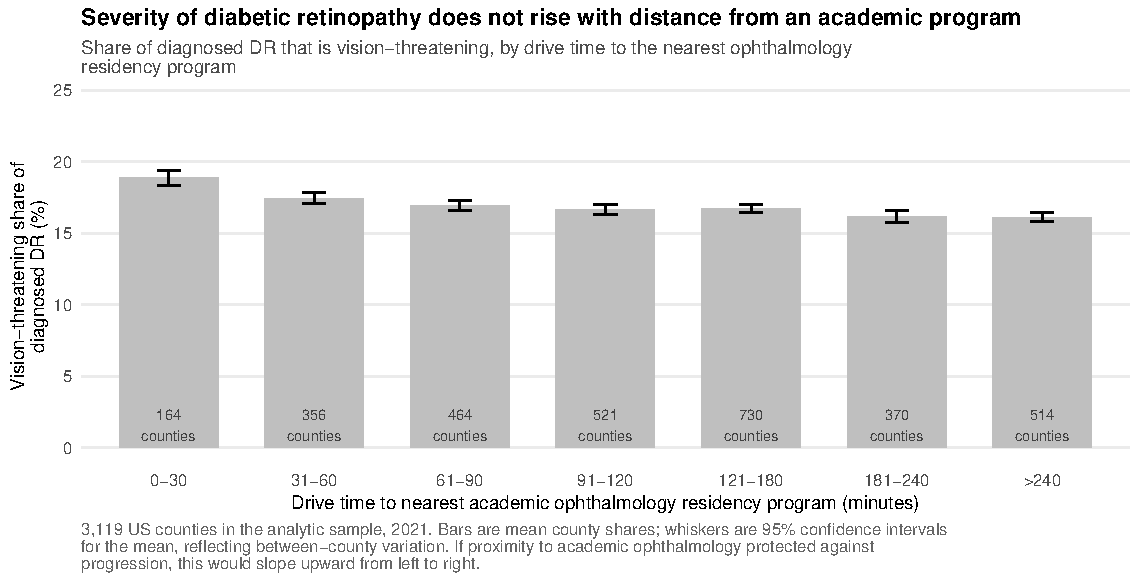
\includegraphics[width=\textwidth]{figs/figA1_drivetime.pdf}
\caption{Vision-threatening share of diagnosed diabetic retinopathy by drive
time to the nearest academic ophthalmology residency program.}
\label{fig:a1}
\end{figure}

\subsection{The association is small, negative, and does not attenuate}

In the within-stratum model the coefficient on log drive time was $-0.017$ per
standard deviation ($P<0.001$). It was essentially unchanged by adjustment for
general eye care proximity, provider density, population density, rurality,
social vulnerability, Medicare diagnostic volume, and preventive screening
completion (Figure~\ref{fig:a3}). A confounded association would be expected to
move toward zero under such adjustment; this one does not, and it points the
wrong way throughout.

\begin{figure}[htbp]
\centering
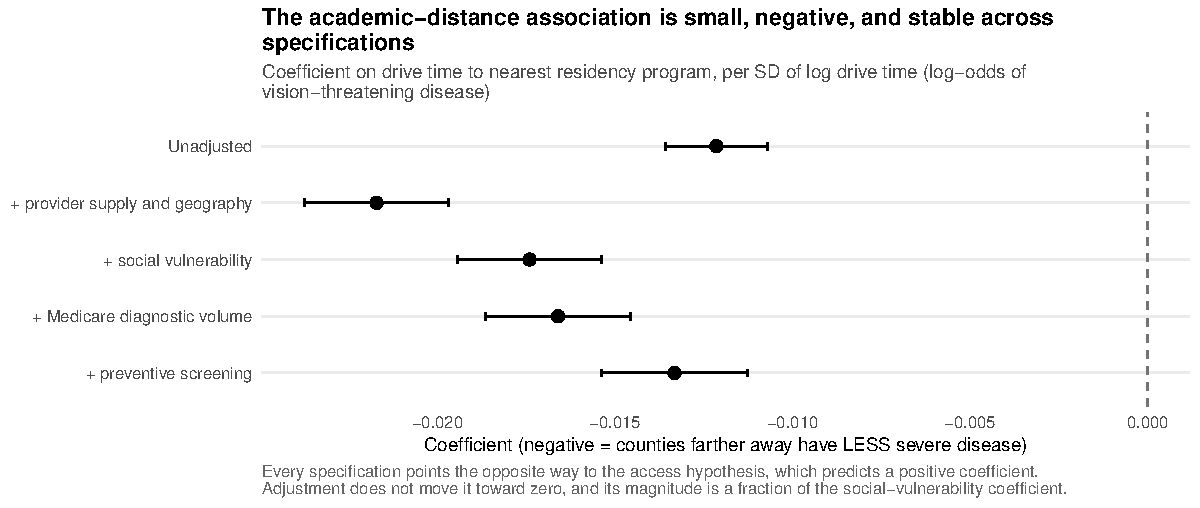
\includegraphics[width=\textwidth]{figs/figA3_forest.pdf}
\caption{Coefficient on drive time to the nearest residency program across
progressively adjusted specifications.}
\label{fig:a3}
\end{figure}

Entered jointly, the two exposures behaved in opposite directions. Distance to
\emph{any} ophthalmologist carried the positive sign an access hypothesis
predicts ($\beta = +0.014$, $P = 0.06$), while distance to an \emph{academic}
program carried a negative one ($\beta = -0.023$, $P<0.001$). The two exposures
correlate at only 0.41 and are therefore separately identified.

\subsection{Discordant counties}

Counties with local ophthalmologists but far from an academic center, the group
whose disadvantage the access hypothesis most directly predicts, did not have
worse case mix: 18.6\% vision-threatening, against 19.6\% among counties with
local ophthalmologists near an academic center (Figure~\ref{fig:a2}). The larger
contrast in the table is horizontal rather than vertical: counties with any
local ophthalmologist had roughly two percentage points \emph{more}
vision-threatening disease than counties with none.

\begin{figure}[htbp]
\centering
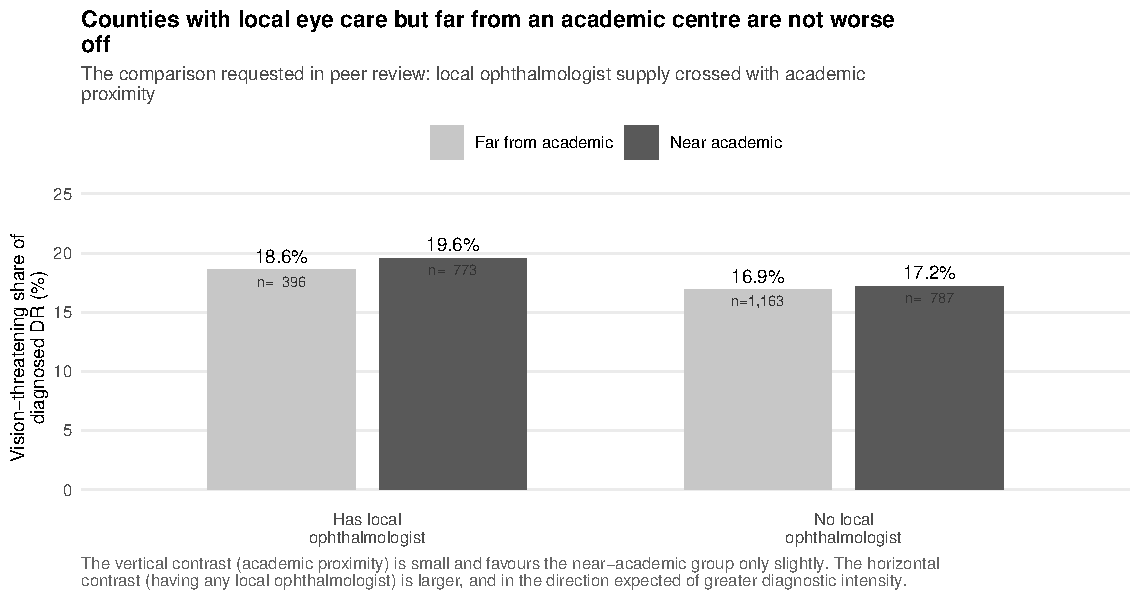
\includegraphics[width=\textwidth]{figs/figA2_discordance.pdf}
\caption{Vision-threatening share by local ophthalmologist supply and academic
proximity.}
\label{fig:a2}
\end{figure}

\subsection{Academic proximity does not matter more where there is no alternative}

If academic centers supply something distinctive, their reach should matter most
where no local eye care exists. The interaction between academic drive time and
having no local ophthalmologist was null ($\beta = 0.008$, $P = 0.70$).
Capacity-weighted access using resident counts performed no better, and was
also wrong-signed ($\beta = +0.010$, $P = 0.06$).

\subsection{Only university program proximity tracks severity}

Distance to the nearest university-based program was associated with the outcome
($\beta = -0.028$, $P<0.001$), whereas distance to the nearest
community-hospital program was associated with nothing at all
($\beta = 0.000$, $P = 0.99$), despite the two distances correlating at 0.61
(Figure~\ref{fig:a4}).

\begin{figure}[htbp]
\centering
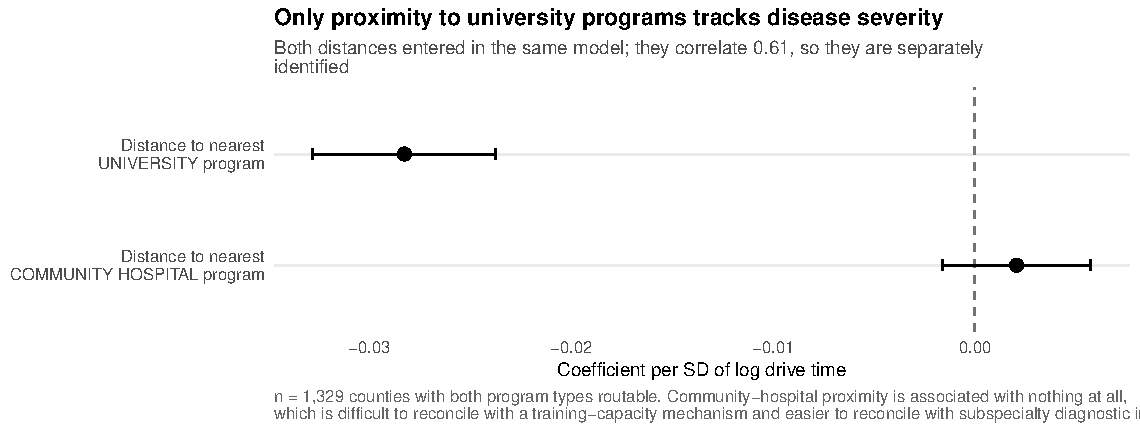
\includegraphics[width=\textwidth]{figs/figA4_progtype.pdf}
\caption{Distance to university-based versus community-hospital programs,
entered jointly.}
\label{fig:a4}
\end{figure}

\subsection{Spatial confirmation}

Residual spatial dependence was substantial (Moran's $I = 0.237$, $P<0.001$).
Under a Leroux conditional autoregressive model fitted to the largest stratum,
the academic drive time posterior mean was $-0.010$ (95\% credible interval
$-0.019$ to $-0.001$), still negative and still small.

%=========================================================================
\section{Discussion}
%=========================================================================

Across every specification we examined, proximity to academic ophthalmology
failed to predict less severe diabetic retinopathy. The association ran in the
opposite direction to the access hypothesis, was small, did not attenuate under
adjustment, was absent where it should have been strongest, and was not improved
by weighting for program capacity.

The most informative single result is the contrast between program types.
Proximity to university-based programs tracked disease severity; proximity to
community-hospital programs, which also train residents, tracked nothing. If the
operative mechanism were training capacity or the presence of an accredited
program, both should behave alike. What distinguishes university departments is
the concentration of subspecialty retinal diagnosis. That is a detection
signature rather than a treatment one.

Several other results point the same way. Counties containing any
ophthalmologist had about two percentage points more vision-threatening disease
than counties with none. Counties with higher Medicare imaging volume had less
vision-threatening disease, consistent with greater diagnostic activity
identifying more mild cases and enlarging the denominator. The authors of the
underlying surveillance estimates anticipated this, cautioning that claims
diagnoses are influenced by access to ophthalmologists and that their model may
mistake such factors for true variation in prevalence.\citep{lundeen2023}

\subsection{Reconciling with clinic-based findings}

Our result appears to contradict Xie et al., who found that patients living more
than eight miles from their ophthalmology clinic had markedly higher odds of
proliferative disease.\citep{xie2025} We do not think the two are in conflict;
they estimate different quantities.

Their exposure is distance to the clinic the patient attended, in a sample of
patients who attended a tertiary referral center. Selection into that sample
depends jointly on distance and on severity: a patient living an hour away is
far more likely to appear in a referral center's records if their disease is
proliferative than if it is mild, because mild disease is managed locally. The
association between distance and severity is therefore partly generated by who
enters the sample. The authors identify this possibility explicitly.

Our design does not condition on attendance. Every county is observed whether or
not its residents travel to a teaching hospital, and the outcome is drawn from
surveillance covering the whole diabetic population rather than from clinic
encounters. Under that design the distance association disappears and reverses.
The natural reading is that the clinic-based association reflects referral
selection rather than a population-level effect of travel burden, and that
inferences about workforce geography should not be drawn from referral-center
samples without a population-level check.

This distinction matters practically. If distance from academic centers caused
proliferative disease, siting new programs would be a rational intervention. If
the clinic-based association is a selection artifact, program placement would be
expected to change where severe disease is \emph{seen} without changing how much
of it there is.

\subsection{What the data do support}

Two findings survive. First, the presence of any local ophthalmologist, not the
academic character of the nearest institution, is what tracks measured disease
severity, and it does so in the direction expected of diagnostic intensity.
Second, in a companion analysis of the same data, county social vulnerability
predicts the vision-threatening share within demographic strata and is
substantially attenuated by general preventive-screening completion, implicating
screening engagement rather than specialty geography.

\subsection{Limitations}

First, this is an ecological analysis; associations cannot be interpreted at the
individual level. Second, the outcome is derived from modeled estimates built on
diagnosed disease in claims, so undiagnosed disease is invisible; this is
precisely the mechanism we invoke to explain the pattern, and we cannot fully
separate it from a true absence of effect. Third, drive times model private
vehicle travel and ignore traffic, ferries, and public transportation entirely;
fourteen island and remote counties in Alaska and Hawaii had no routable path
and are excluded. Fourth, the university versus community contrast is estimated
on 1,333 counties having both program types among their routed candidates, a
subsample skewed urban and eastern. Fifth, residency program location is a proxy
for academic ophthalmology and does not capture non-academic retina practices,
satellite clinics, or teleretinal programs. Sixth, Puerto Rico is absent from the
VEHSS source.

\subsection{Conclusion}

At the population level, counties farther from academic ophthalmology do not
carry more vision-threatening diabetic retinopathy. The geography of academic
ophthalmology appears to shape where advanced disease is detected rather than
how much of it occurs. Strategies aimed at reducing preventable vision loss are
better directed at screening completion within disadvantaged communities than at
the geographic placement of training programs.

\clearpage

%=========================================================================
\begin{thebibliography}{99}

\bibitem[American Academy of Ophthalmology(2024)]{aao2024ppp}
American Academy of Ophthalmology. \emph{Diabetic Retinopathy Preferred Practice
Pattern}. 2024.

\bibitem[Berkowitz et al.(2024)]{berkowitz2024}
Berkowitz ST, Finn AP, Parikh R, Kuriyan AE, Patel S. Ophthalmology workforce
projections in the United States, 2020 to 2035. \emph{Ophthalmology.}
2024;131(2):133--139.

\bibitem[Centers for Disease Control and Prevention(2024a)]{vehss}
Centers for Disease Control and Prevention. Vision and Eye Health Surveillance
System: composite prevalence estimates. \url{https://data.cdc.gov/resource/qeru-k2y2}.
Accessed August 2026.

\bibitem[Centers for Disease Control and Prevention(2024b)]{svi}
CDC/Agency for Toxic Substances and Disease Registry. Social Vulnerability Index
2020, county level. \url{https://svi.cdc.gov}. Accessed August 2026.

\bibitem[Centers for Medicare \& Medicaid Services(2021)]{cmsgeo}
Centers for Medicare \& Medicaid Services. Medicare Geographic Variation by
National, State \& County, 2021. \url{https://data.cms.gov}. Accessed August 2026.

\bibitem[County Health Rankings(2021)]{chr}
University of Wisconsin Population Health Institute. County Health Rankings \&
Roadmaps 2021 analytic data. \url{https://www.countyhealthrankings.org}.
Accessed August 2026.

\bibitem[Feng et al.(2020)]{feng2020}
Feng PW, Ahluwalia A, Feng H, Adelman RA. National trends in the United States
eye care workforce from 1995 to 2017. \emph{Am J Ophthalmol.} 2020;218:128--135.

\bibitem[Health Resources and Services Administration(2023)]{ahrf}
Health Resources and Services Administration. Area Health Resources Files,
2022--2023 release. \url{https://data.hrsa.gov}. Accessed August 2026.

\bibitem[Lundeen et al.(2023)]{lundeen2023}
Lundeen EA, Burke-Conte Z, Rein DB, et al. Prevalence of diabetic retinopathy in
the US in 2021. \emph{JAMA Ophthalmol.} 2023;141(8):747--754.

\bibitem[Soares et al.(2023)]{soares2023}
Soares RR, Mokhashi N, Sharpe J, et al. Patient accessibility to eye care in the
United States. \emph{Ophthalmology.} 2023;130(4):354--360.

\bibitem[US Census Bureau(2021)]{cenpop}
US Census Bureau. Centers of Population by County, 2020 Census.
\url{https://www2.census.gov/geo/docs/reference/cenpop2020/}. Accessed August 2026.

\bibitem[Weng et al.(2024)]{weng2024}
Weng CY, Maguire MG, Flaxel CJ, et al. Effectiveness of conventional digital
fundus photography-based teleretinal screening for diabetic retinopathy and
diabetic macular edema. \emph{Ophthalmology.} 2024;131(8):927--942.

\bibitem[Xie et al.(2025)]{xie2025}
Xie WY, Rustam Z, Tran D, et al. Association of neighborhood socioeconomic
disadvantage with proliferative diabetic retinopathy. \emph{Ophthalmol Retina.}
2025;9(2):e1--e9. doi:10.1016/j.oret.2024.10.012

\end{thebibliography}

\end{document}
